\chapter{Dynkin Diagrams}
\label{ch-dynkin}

\newcommand{\valp}[0]{{\vec{\alp}}}
\newcommand{\vbeta}[0]{{\vec{\beta}}}
\newcommand{\vgamma}[0]{{\vec{\gamma}}}

This chapter is based on Ref.\cite{eli-daw-book}, section 20.4.

This chapter is an overview of the classification
of simple Lie algebras, a classification that was invented mainly by Killing, Cartan and Dynkin, in that historical order. The classification is valid for Lie algebras over $\CC$\footnote{More generally, Cartan's classification is valid for Lie algebras over $\FF$, where $\FF$ is an algebraically closed field of characteristic zero. $\CC$ satisfies both of these constraints. $\RR$ has characteristic zero but is not algebraically closed.} This caveat is important because there are more simple Lie algebras over $\RR$ than over $\CC$. When defining the generators of Lie algebras in other chapters, we defined a real Lie algebra $\ger{g}_\RR$ (a vector space over $\RR$)
which exponentiates to a group $\calg_\RR=\exp(\ger{g}_\RR)$.
This chapter refers to the complexification
$\ger{g}_\CC$  (a vector space
over $\CC$) of $\ger{g}_\RR$ 
and to the group $\calg_\CC=\exp(\ger{g}_\CC)$


Suppose $\ger{g}_\CC$ has generators $X_s$ for
$s\in S=\{1,2, \ldots \cald\}$ where 

$\cald=\frac{1}{2}\dim_\RR \ger{g}_\CC=\dim_\CC \ger{g}_\CC=$  half the number  of real degrees of freedom
of the Lie algebra.

By definition,
the generators $X_s$ are closed under commutation so
\beq
[X_q, X_p] = \sum_t f\indices{_q_p^t}X_t
\eeq
for some $f\indices{_q_p^t}\in \CC$.

Define
\beq
g_{qs}= \sum_{p,t}f\indices{_q_p^t}
f\indices{_s_t^p}
=
\bcen
\xymatrix{
q\ar@{~}[r]
&f\ar@/_1pc/@{~}[r]
\ar@/^1pc/@{~}[r]
&f\ar@{~}[r]
&s
}
\ecen
\eeq
If $\det g =0$,
we can find disjoint sets $S_1$, $S_2$ so that $S=S_1\cup S_2$ and

\beq
[X_{a}, X_{b}] = 0\quad \text {for $a,b\in S_1$}
\eeq
and
\beq
[X_q, X_p] =\sum_t f\indices{_q_p^t}X_t
\quad \text {for $p,q,t\in S_2$}
\eeq

{\bf Cartan Criterion:} $\det g \neq 0$ 

We will assume that the CC is satisfied. This implies that
the Lie algebra is semi-simple and 
that we can and will assume that 
$g_{st}$ is diagonal.

\beq g_{s t}=\delta(s,t)=
\xymatrix{
\ar@{~}[r]&
}
\eeq

\beq
f\indices{_q_p^t}=f_{qpt}
\eeq
Will not, however, assume that $f_{qpt}$ 
is totally antisymmetric,
as is often assumed.

\hrule
Cartan-Weyl commutators for $\ger{su}(2)$

\beq
E_-=\ket{2}\bra{1} , \quad E_+=\ket{1}\bra{2},
\quad H= \frac{1}{2}[\ket{1}\bra{1}-\ket{2}\bra{2}]
\label {eq-su2-norm-op}
\eeq

\beq
\begin{array}{ll}
\bcen
\xymatrix{
&H\ar[dl]_{-E_-}
\ar[dr]^{E_+}
\\
E_-&&E_+\ar[ll]^{2H}
}
\ecen
&
\left\{
\begin{array}{l}
[E_+, E_-]=2H
\\
{[H, E_+]=E_+}
\\
{[H,, E_-]=-E_-}
\end{array}
\right.
\end{array}
\eeq
\hrule
Cartan-Weyl commutators for any semi-simple Lie algebra

For any lower case latin letter $q$ and Greek letter $\alp$, let

$q_- = 1, 2, \ldots,\calr$

$\valp = \calr+1,\calr+2, \ldots, 
\cald$ 

$q=$ either $q_-$ or $\valp$ but not both.

Let $\{H_{i_-}\}_{i_-=1}^\calr$
be the largest possible set
of mutually commuting $X_p$.
$\calr$ is called the {\bf rank} of the group.

\beq
\boxed{[H_{i_-}, H_{j_-}]=0}
\eeq

Let $E_{\vec{\alp}}$
 be eigenvectors of $H_{i_-}$ 
for a commutator \qt{product}
instead of a matrix multiplication product
\beq
\boxed{[H_{i_-}, E_{\vec{\alp}}]= \alp_{i_-}E_{\valp}}
\eeq
The vectors $\valp\in \RR^\calr$
of eigenvalues are called {\bf root vectors}.


From the properties of a commutator bracket\footnote{The commutator $[x,y]=xy-yx$ acts like a derivative operator: 
$ [x[a,b]]= [[x,a],b] + 
[a,[x,b]]$}


\beqa
[H_{i_-}, [E_\valp,
E_\vbeta]]
&=&
[[H_{i_-}, E_\valp], E_\vbeta]
+
[E_\valp, [H_{i_-}, E_\vbeta]]
\\
&=&
(\alp_{i_-} + \beta_{i_-})[E_\valp, E_\vbeta]
\eeqa


If $\valp + \vbeta=0$,
$[H_i, [E_\valp,
E_\vbeta]]=0$ so

\beq
\boxed{[E_\valp,
E_{-\valp}] = \sum_{i_-} \xi_{i_-}H_{i_-}}
\eeq
\begin{claim}
If we assume the normalization of $\ger{su}(2)$
operators used in Eq.(\ref{eq-su2-norm-op}), the
\beq
\xi_{i_-}=\frac{2\alp_{i_-}}{\vec{\alp}\cdot \vec{\alp}}
\eeq
\end{claim}
\proof
Let $E_\valp \rarrow E_+$, $E_{-\valp}\rarrow E_-$, $|\valp|=1$.

\qed

If $\valp + \vbeta\neq 0$,

\beq
\boxed{[E_\valp, E_\vbeta]=
 N_{\valp,\vbeta}
E_{\valp + \vbeta}
\quad \text{ if } \valp+\vbeta \neq 0}
\eeq
for some $N_{\valp,\vbeta}\in \CC$.


The roots ({\bf root system}) of a semisimple Lie algebra form a
real $\calr$ dimensional vector space.

A {\bf positive/negative (P/N) root} $\valp$ is a
root for which the first component $\alp_1$ is positive/negative.
If the first component of $\valp$ is zero, then
decide the root's sign from its second component $\alp_2$. And so on.
Note that the definition of P/N root is basis
dependent.

A P root $\valp$ is a {\bf simple positive (SP)
root} if there are no P roots
$\vec{\rho}$ and $\vec{\s}$ such that
$\valp= \vec{\rho}+\vec{\s}$.
Hence, SP roots are like
the atoms or indivisible 
constituents of the root system.




Properties of root vectors $\valp, \vbeta, \ldots \in \RR^\calr$ 



\begin{enumerate}
\item If $\valp$ is a root,  then
$-\valp$ is too.


\item We can find a basis of SP roots for the root space.


\item 
\begin{claim}If $\valp$ and $\vec{\rho}$ are SP roots,
then $\valp-\vec{\rho}$ is not a root of any kind.
\end{claim}
\proof

Assume $\valp-\vec{\rho}$ is either a P root or an N root. 

If $\valp-\vec{\rho}$ is a P root
 $\vec{\s} $, then
$\valp= \vec{\rho}+\vec{\s}$ so
$\valp$ is not a SP root. 

Likewise, if $\valp-\vec{\rho}$ is an N root $\vec{\s}$, then $-\vec{\s}$
is a P root and $\valp= \vec{\rho}+(-\vec{\s})$.
\qed



\item If $\valp$ and $\vbeta$ are SP, then there can be roots 

\beq\{\vbeta + n\valp| 
i=0, 1, 2, \ldots, n\}
\eeq
for some terminal integer $n\geq 0$ defined by (see Fig.\ref{fig-dynkin-constraint})
\beq 
n= \frac{-2 \valp\cdot \vbeta}{\valp\cdot\valp}
\label{eq-dynkin-n-pic}
\eeq
The following roots are
also possible \beq\{\valp + p\vbeta| 
i=0, 1, 2, \ldots, p\}\eeq
for some terminal integer $p\geq 0$ defined by (see Fig.\ref{fig-dynkin-constraint})


\beq 
p= \frac{-2 \valp\cdot \vbeta}{\vbeta\cdot\vbeta}
\label{eq-dynkin-p-pic}
\eeq



\item angle constraint

Multiplying Eqs.(\ref{eq-dynkin-n-pic}) and
(\ref{eq-dynkin-p-pic}), we get
\beq
-\sqrt{
\frac{np}{4}}
=
\hat{\alp}\cdot\hat{\beta}\in [-1, 0]
\label{eq-dynkin-angles}
\eeq
This angle constraint
implies that the angle
between the two SP roots $\valp$
and $\vbeta$ can only
have one of the 4 possible values listed in Table \ref{tab-dynkin-angles}.

\item length ratio constraint

Dividing Eqs.(\ref{eq-dynkin-n-pic}) and
(\ref{eq-dynkin-p-pic}), we get
\beq
\sqrt{\frac{n}{p}}=\frac{|\vbeta|}
{|\valp|}
\label{eq-rel-len-cons}
\eeq
Table \ref{tab-rel-len-cons}
gives the possible length ratios implied by Eq.(\ref{eq-rel-len-cons}).
\end{enumerate}

\begin{figure}[h!]
\centering
\includegraphics[width=5in]
{dynkin/dynkin-constraint.png}
\caption{Pictorial representation of 
Eqs.(\ref{eq-dynkin-n-pic})
and (\ref{eq-dynkin-p-pic}).
}
\label{fig-dynkin-constraint}
\end{figure}

\begin{table}[h!]
\begin{tabular}{|l|l|l|}
\hline
\rowcolor[HTML]{FFFFC7} 
$np$ & $\sqrt{np/4}$ & $\angle(\valp, \vbeta)=\arccos\left(-\sqrt{np/4}\right)$ \\ \hline
0 & 0 & $\frac{\pi}{2}=90^o$ \\ \hline
1 & $\frac{1}{2}$ & $\frac{2\pi}{3}=120^o$ \\ \hline
2 & $\frac{1}{\sqrt{2}}$ & $\frac{3\pi}{4}=135^o$ \\ \hline
3 & $\frac{\sqrt{3}}{2}$ & $\frac{5\pi}{6}=150^o$ \\ \hline
\end{tabular}
\caption{The 4 possible angles between two PS roots, as dictated by the angle
constraint  Eq.(\ref{eq-dynkin-angles}).}
\label{tab-dynkin-angles}
\end{table}

% Please add the following required packages to your document preamble:
% \usepackage[table,xcdraw]{xcolor}
% Beamer presentation requires \usepackage{colortbl} instead of \usepackage[table,xcdraw]{xcolor}
\begin{table}[h!]
\begin{tabular}{|l|l|l|}
\hline
\rowcolor[HTML]{FFFFC7} 
$np$ & $(n,p)$ & $|\vbeta|/|\valp|$ \\ \hline
0 & (0, 1) or (1,0) & 0 or $\infty$ \\ \hline
1 & (1,1) & 1 \\ \hline
2 & (1,2) or (2,1) & $1/\sqrt{2}$ or $\sqrt{2}$ \\ \hline
3 & (1,3) or (3,1) & $1/\sqrt{3}$ or $\sqrt{3}$ \\ \hline
\end{tabular}
\caption{Possible length ratios between two PS roots, as dictated by the length ratio constraint Eq.(\ref{eq-rel-len-cons}).}
\label{tab-rel-len-cons}
\end{table}

Using the definition of SP roots, and the angle and length constraints on SP roots,
one can show that all possible 
simple Lie algebras 
have one of the root systems given by Fig.\ref{fig-dynkin-simple}.  In that figure,
the parameters of a root
system are specified via 
Dynkin diagrams.

Rules for drawing {\bf Dynkin Diagrams (DD)}
\begin{enumerate}
\item One dot for each SP root. $k$ subscript in $A_k, B_k, C_k, D_k$
is number of dots
\item Dots connected by $np$ number of lines
\item If $np>1$, draw arrowhead (i.e., greater-than sign $>$) pointing from bigger to smaller root.

\item Draw one connected diagram (CD) for a simple Lie algebra. Draw multiple disconnected CDs for a semisimple Lie algebra. 

This follows because the Lie algebra of a semisimple Lie algebra $\ger{g}$ is a direct sum $\ger{g}= \ger{g}_1 \oplus \ger{g}_2 \oplus \ldots \ger{g}_t$
of simple Lie algebras $\ger{g}_i$ and the root vectors
of any two of those Lie algebras $\ger{g}_1$ and $\ger{g}_2$ are orthogonal so
$np=0$ and 
there is no line connecting the roots of $\ger{g}_1$ and $\ger{g}_2$. 
\end{enumerate}



\begin{figure}
\renewcommand{\arraystretch}{2}
$$
\begin{array}{ll}
 A_k=\ger{su
}(k+1)
& \dynkin[scale=3]A{}
\\
B_k=\ger{so}(2k+1)
& \dynkin[scale=3]B{}
\\
C_k=\ger{sp}(2k) 
&\dynkin[scale=3] C{}
\\
D_k=\ger{so}(2k) 
& \dynkin[scale=3] D{}

\\ E_6& \dynkin[scale=3] E6{}

\\ E_7& \dynkin[scale=3] E7{}

\\ E_8 &\dynkin[scale=3] E8{}

\\ F_4 & \dynkin[scale=3] F4{}

\\ G_2 & \dynkin[scale=3] G2{}

\end{array}
$$
\renewcommand{\arraystretch}{1}
\caption{Dynkin diagrams for the simple Lie groups.
$n$ subscript in $A_k, B_k, C_k, D_k$
is the number of dots, which equals the number of SP roots.}
\label{fig-dynkin-simple}
\end{figure}

\section{Examples}


\begin{itemize}
\item DD for $SO(3)$ and its double cover $SU(2)$ is a single dot

\item $SO(4)\cong SO(3)\times SO(3)$ is not a simple Lie algebra.  Its DD is two disconnected dots

\item For $SU(3)$, the DD is $\xymatrix{\bullet\ar@{-}[r]&\bullet}$

\beq
H_1=T_z,\quad H_2=\frac{\sqrt{3}}{2} Y
\eeq

\beq
E_\valp= \frac{1}{\sqrt{2}} T_+,
\quad
E_\vbeta = \frac{1}{\sqrt{2}} U_+,
\quad
E_{\vec{\alp}+\vec{\beta}}=\frac{1}{\sqrt{2}} V_-
\eeq


\begin{figure}[h!]
\centering
\includegraphics[width=2in]
{dynkin/dynkin-su3-roots.png}
\caption{Root system for $SU(3)$}
\label{fig-su3-roots}
\end{figure}


\end{itemize}



